\documentclass[12pt,a4paper,oneside]{article}
\usepackage[colorlinks=true, unicode]{hyperref}
\usepackage[utf8]{inputenc}
\usepackage[czech]{babel}
\usepackage{graphicx}
\usepackage{pdfpages}
\textwidth 16cm \textheight 25cm
\topmargin -1.3cm 
\oddsidemargin 0cm
\usepackage{footnote}
\pagestyle{empty}
\begin{document}
\title{I$^2$C Světelný seznor }
\author{Jakub Kákona, kaklik@mlab.cz}
\maketitle

\thispagestyle{empty}
\begin{abstract}
Senzor osvětlení ve viditelném a IR spektru. 
\end{abstract}

\begin{figure} [htbp]
\begin{center}
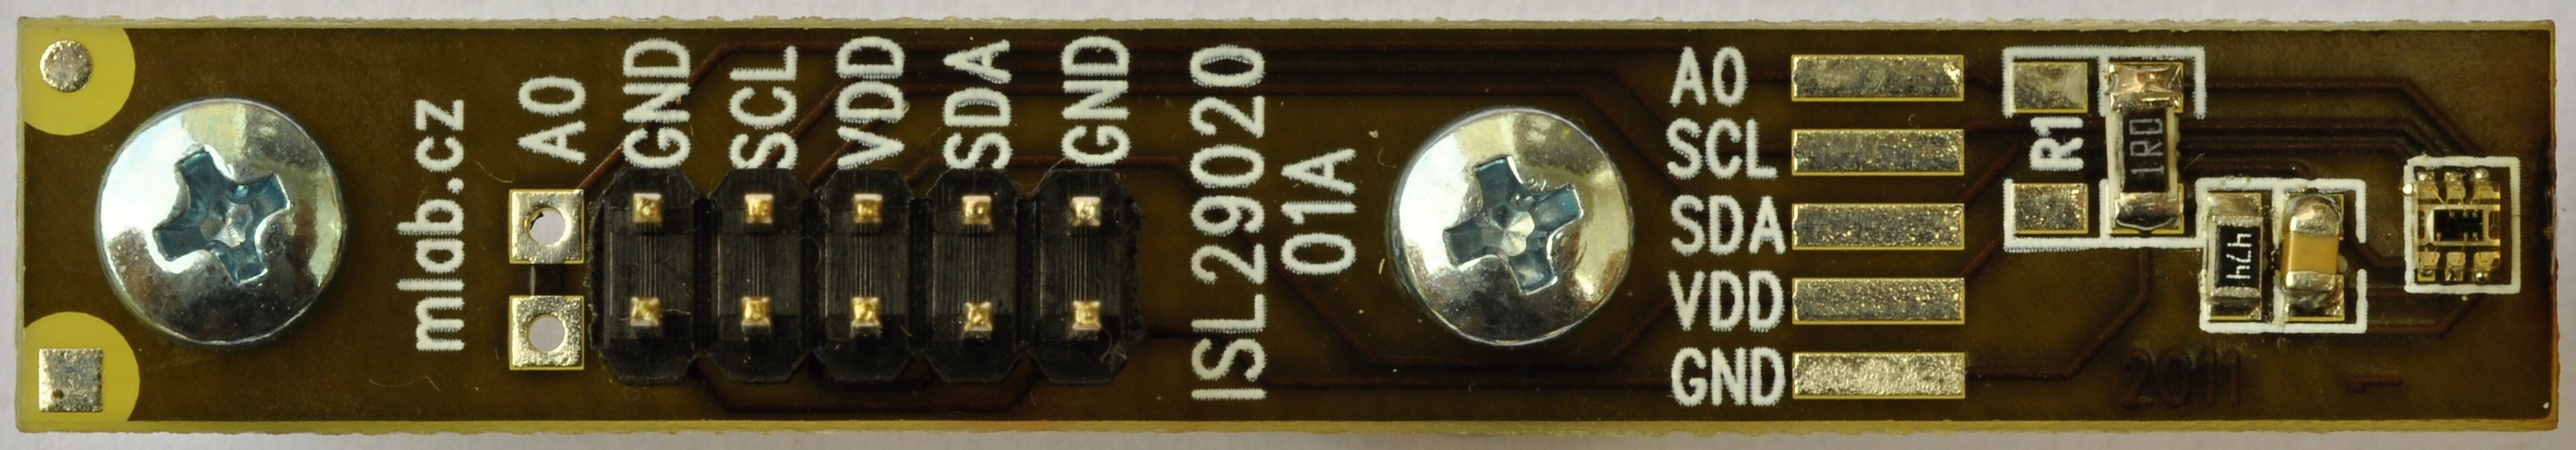
\includegraphics [width=100mm] {./img/ISL2902001A_Top_Big.jpg} 
\end{center}
\end{figure}

\begin{figure} [b]

\includegraphics [width=25mm] {./img/ISL2902001A_QRcode.png} 
\end{figure}

\newpage
\tableofcontents

\section{Technické parametry}
\begin{table}[htbp]
\begin{center}
\begin{tabular}{|c|c|p{4.7cm}|}
\hline
Parametr & Hodnota & Poznámka \\
\hline
Napájecí napětí  & max 3.6V & \\ 
\hline
Digitální úrovně &  I2C &  Odpovídají napájecímu napětí. \\ 
\hline
Měřící rozsah &  0-40k Lux &   \\ 
\hline
\end{tabular}
\end{center}
\end{table}

\section{Popis konstrukce}

\subsection{Zapojení}

Zapojení modulu je realizováno pouze blokovacím kondenzátorem a možností výběru ze dvou adres osazením jednoho ze dvou rezitorů. Rezistorem R3 je pak možné změnit integrační konstantu měřícího obvodu. Hodnota v osazovacím plánu je zvolena tak, aby výsledné měřené hodnoty měly rozměrměr Lux. 

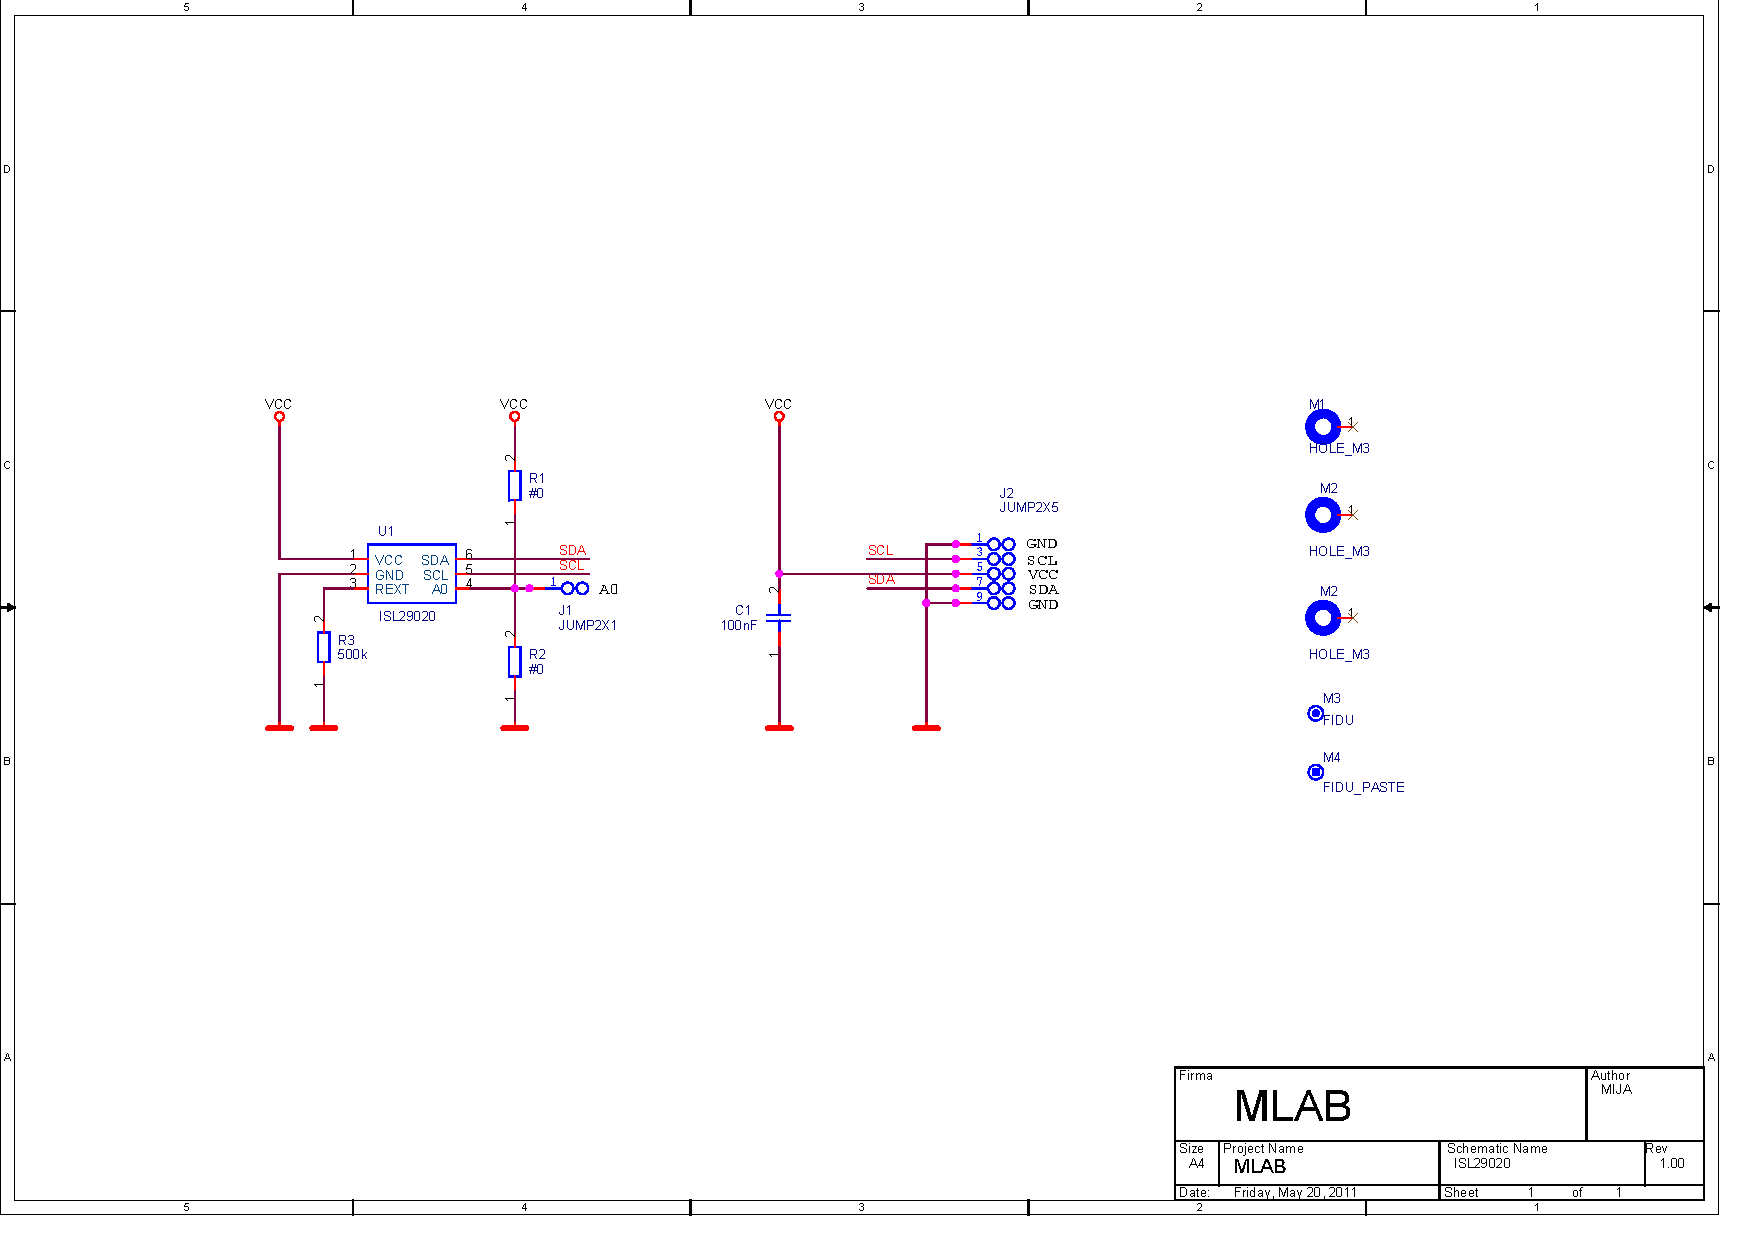
\includepdf[pages={1},landscape=false]{../../SCH/ISL29020.pdf}

\subsection{Mechanická konstrukce}

Konstrukčně je modul řešen tak, že předpokládá uchycení na dvou šroubech mimo osu měřenéhého záření. Může být proto uchycen na desku v krabičce a měřené čidlo může přečnívat mimo základní desku. 

\section{Výroba a testování}

Plošný spoj je navržen pro osazování pomocí pasty.  Modul se testuje optickou kontrolou spojů a následným připojením na laboratorní zdroj s omezením proudu a  vyčtením digitálních hodnot ze senzoru. 

\newpage

\begin{figure} [h!tbp]
  \centering
  %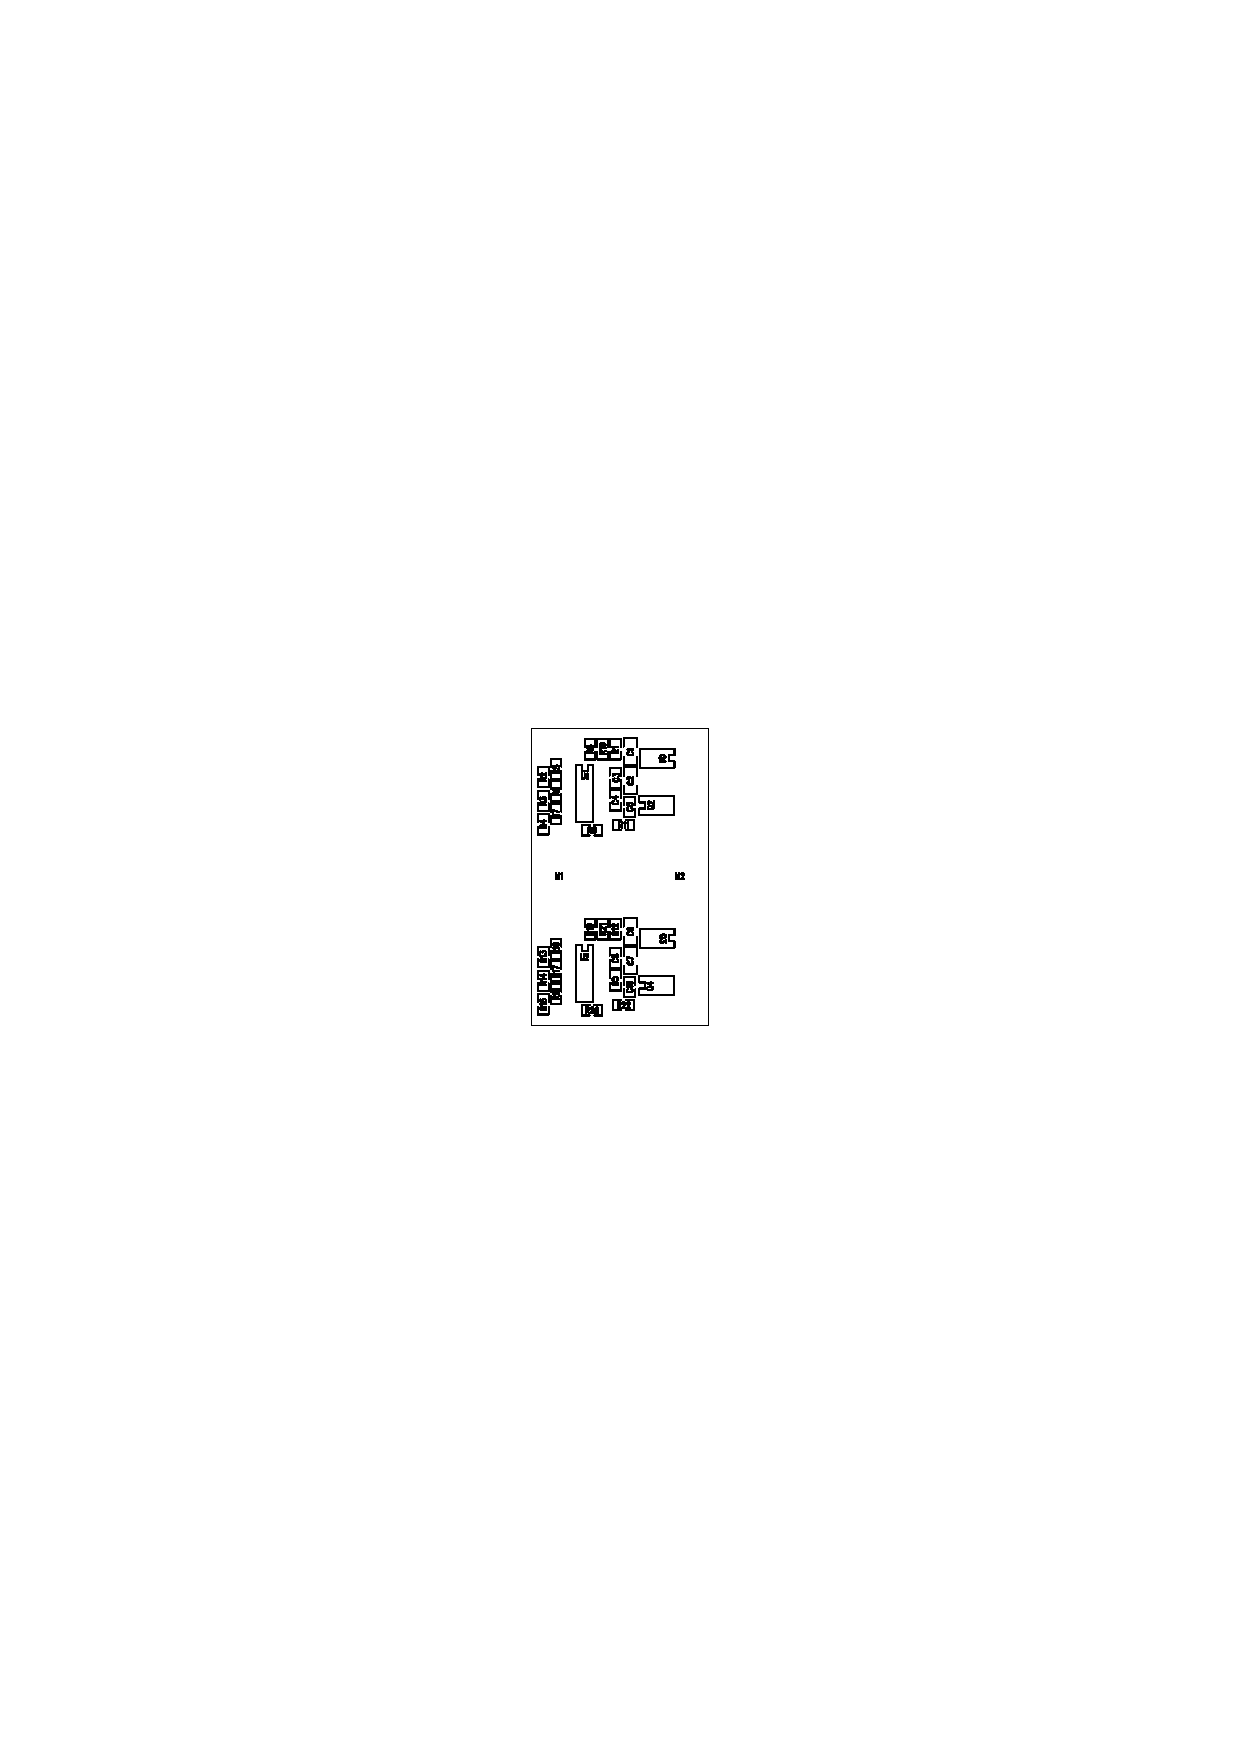
\includegraphics[trim = 7.0cm 12.0cm 7.0cm 12.0cm, clip, width=12cm]{../../CAM_DOC/O1.pdf}
  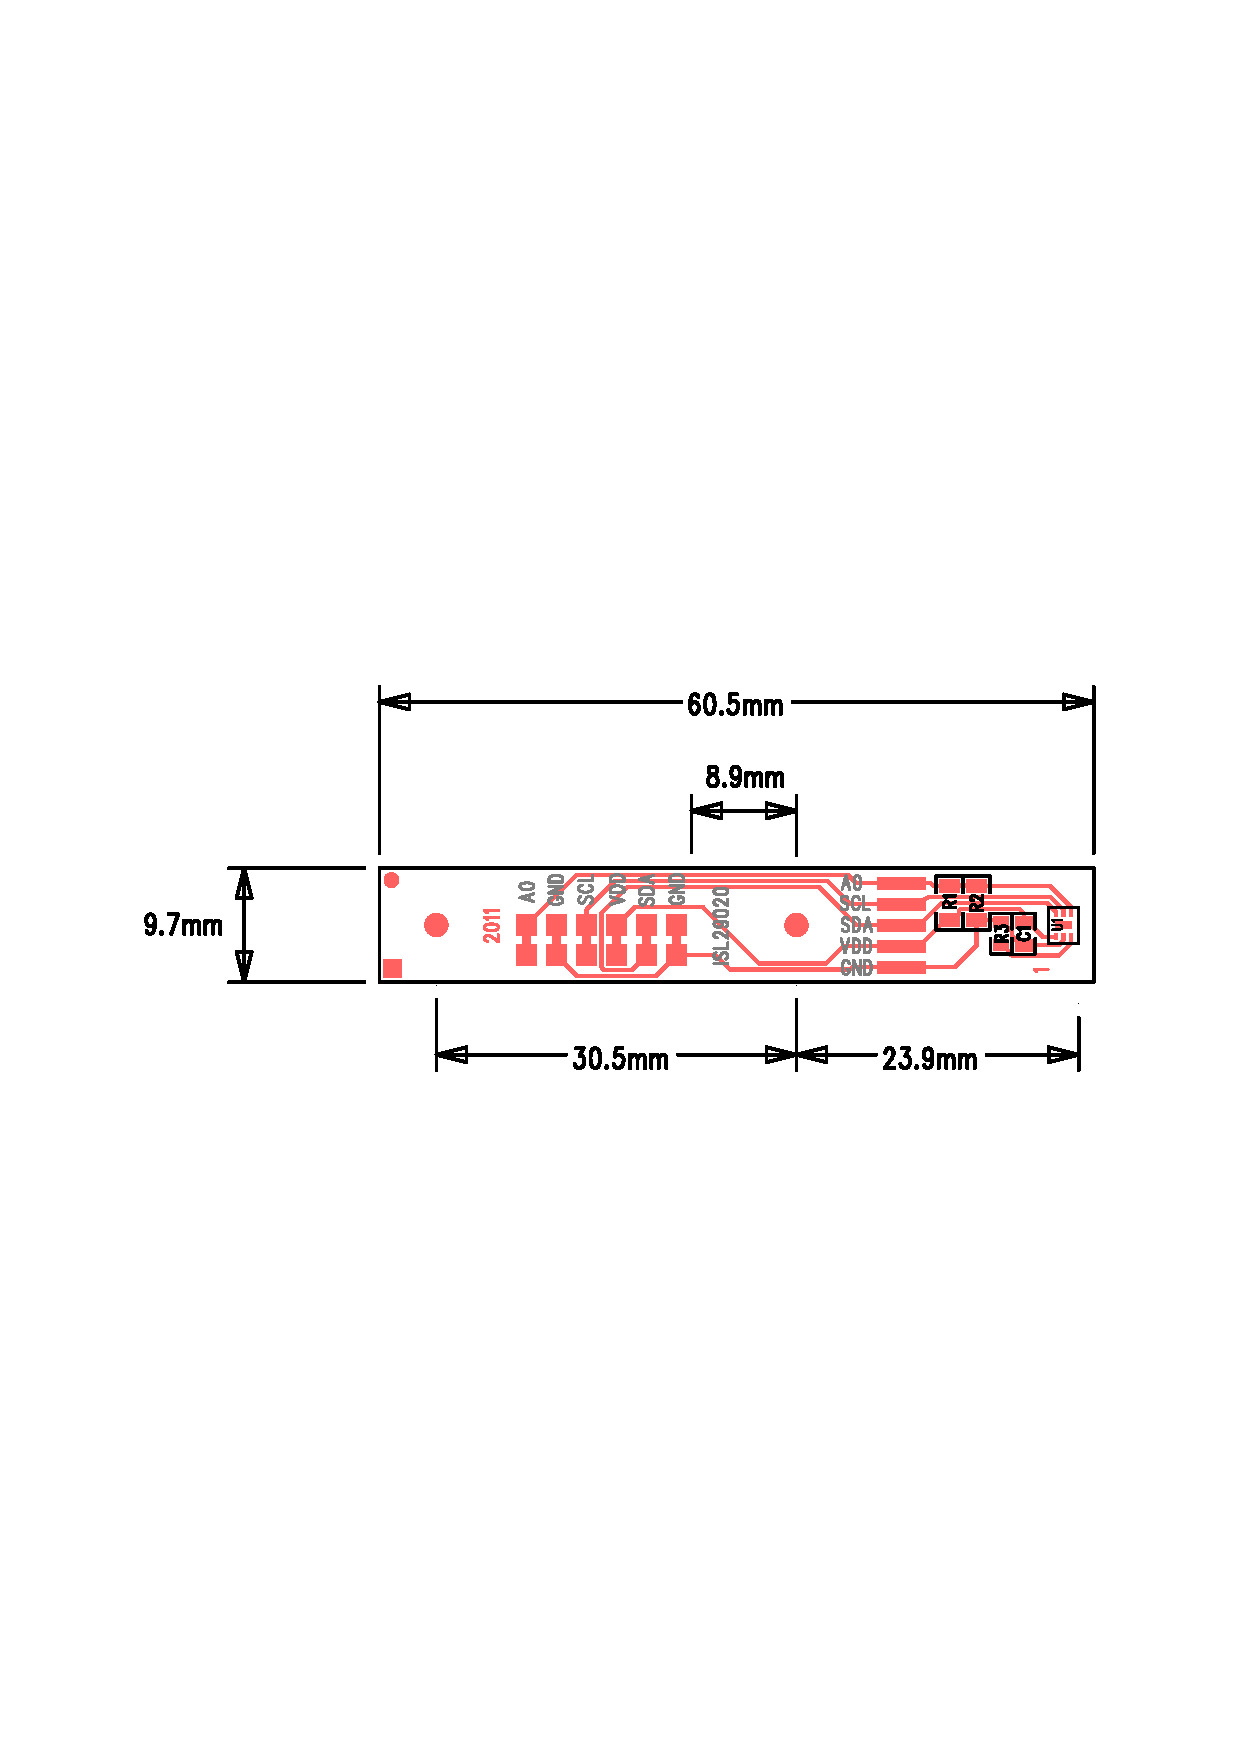
\includegraphics[trim = 2.0cm 10.5cm 2.0cm 10.5cm, clip, width=12cm]{../../CAM_DOC/O2.pdf}
  \caption{Osazovací plán horní a spodní strany plošného spoje}
  \label{fig:osazovaci_plan}
\end{figure}

\begin{savenotes}
\begin{table}[h!]
\begin{center}
\begin{tabular}{ |c|c|c|c| }
\hline 
Počet & Označení & Typ  & Pouzdro  \\ 
\hline 
1	&	C1	&	100nF	&	0805	\\
1	&	J1	&	JUMP2X1	&		\\
1	&	J2	&	JUMP2X5	&		\\
2	&	R1,R2	&	1x 0R	&	0805	\\
1	&	R3	&	500k	&	0805	\\
1	&	U1	&	ISL29020	&	\\
\hline 
\end{tabular}
\end{center}
\caption{Seznam součástek potřebných pro osazení modulu.}
\label{seznam_soucastek}
\end{table}
\end{savenotes}

\newpage

\section{Programové vybavení}

V MLAB Python knihovně Pymlab je testovací příklad k seznoru. 

\begin{thebibliography}{99}

\end{thebibliography}
\end{document}